\section{Einleitung}
% In diesem Versuch soll die Relaxationszeit von Dipolen in Kristallen vermessen werden.
%
In diesem Versuch werden die Leitungseigenschaften von verschiedenen Koaxialkabeln vermessen.


\section{Koaxialkabel}
\label{sec:koax}
Koaxialkabel werden zur störungsfreien Übertragung von hochfrequenten Signalen genutzt.
Sie bestehen aus einem Leiter im Inneren, einer Isolationsschicht und einer weiteren Leitungsschicht außen.
Durch die äußere Schicht werden externe Störsignale abgeschirmt.
In Abbildung \ref{fig:koax} ist der Querschnitt durch ein Koaxialkabel dargestellt.
Eingezeichnet sind außerdem die Richtungen der Feldkomponenten des Elektrischen und Magnetischen Felds $\vec{E}$ und $\vec{H}$.
\begin{figure}
  \centering
  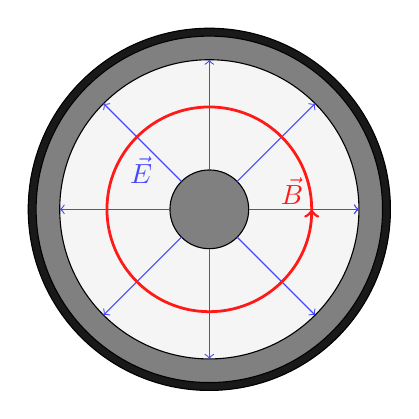
\begin{tikzpicture}
\draw [fill=black!90] (0,0) circle [radius=2.3];
\draw [fill=gray] (0,0) circle [radius=2.2];
% \draw [black] (0,0) circle [radius=2];
\draw [fill=black!4] (0,0) circle [radius=1.9];
\draw [fill=gray] (0,0) circle [radius=0.5];
\foreach \y in {0,45,90,...,360}
{

       \draw [blue!80!white!90, ->] (\y:0.5) -- (\y:1.9);
      %  \pgfmathtruncatemacro{\cur}{\x + 5* \y}
      %  \pgfmathtruncatemacro{\next}{\cur + 1}
      %  \draw (\cur) -- (\next);
}

\draw [red!90,->,line width=1pt] (1.3,0) arc [radius=1.3, start angle=0, end angle= 360];
\node [red!90]at (1.05,0.23) {$\vec{B}$};

\node [blue!80!white!90]at (150:1.0) {$\vec{E}$};

\end{tikzpicture}

  \caption{Schematische Darstellung eines Koaxialkabels.}
  \label{fig:koax}
\end{figure}

Das elektrische Feld breitet sich radial vom Innen- zum Außenleiter aus.
Das Magnetfeld läuft an jeder Stelle orthogonal zum E-Feld kreisförmig um den inneren Leiter.
An das Koaxialkabel werden Wechselspannungen angelegt.
Solang eine materialabhängige Grenzfrequenz nicht überschritten wird breiten sich dann die Felder in dem Kabel
wellenförmig aus.
Die Ausbreitungsrichtung der Wellen, also die des Energie- und Informationsübertrags, geht in Richtung des Poynting-Vektors.
Dieser ist definiert als
\begin{equation}
  \label{eq:poynting}
  \vec{S} = \vec{E} \times \vec{B}.
\end{equation}
Durch das Kreuzprodukt steht der Poynting-Vektor immer senkrecht auf den Feldern. In der Zeichnung steht er also senkrecht
zur Bildfläche.

Zwischen den leitenden Elementen des Kabels entsteht durch Potentialunterschied eine Kapazität $C$.
Abhängig vom Material welches für die Isolationsschicht verwendet wird, entsteht eine Induktivität $L$.
Das Koaxialkabel kann durch die Ersatzschaltung in Abbildung~\ref{fig:circuit} dargestellt werden.
\begin{figure}
  \centering
  \begin{circuitikz}[american voltages]
\draw
  % stator circuit
  (0,0) to [open, v^>=$U$] (0,3) %
  to [short, *- ] (2,3) %
  % to [R, l=$R_L$] (3,3) %
  to [L, l=$L$] (6,3) %
  to [C, l=$C$] (6,0) %

  (6,3)    to [short, -*] (10,3) %

  (0,0) to [short, *-*] (10,0);
\end{circuitikz}

  \caption{Ersatzschaltbild eines optimalen Koaxialkabels.}
  \label{fig:circuit}
\end{figure}

In einem physikalischen Leiter kommt es außerdem zu Ohmschen Verlusten. Zu dem Ersatzschaltbild müssen demnach noch Widerstände hinzugefügt werden.
\begin{figure}
  \centering
  \begin{circuitikz}[american voltages]
\draw
  % stator circuit
  (0,0) to [open, v^>=$U$] (0,3) %
  to [short, *- ] (2,3) %
  to [R, l=$R_L$] (3,3) %
  to [L, l=$L$] (5,3) %
  to [R, l=$G$] (5,0) %
  (7,3) to [C, l=$C$] (7,0) %
  (5,3)    to [short, -*] (10,3) %

  (0,0) to [short, *-*] (10,0);
\end{circuitikz}

  \caption{Ersatzschaltbild eines Koaxialkabels mit ohmschen Verlusten.}
  \label{fig:circuit_ohm}
\end{figure}


\subsection{Telegraphengleichung}
Die Ausbreitung der elektromagnetischen Wellen kann durch die Telegraphengleichung beschrieben werden.
Es handelt sich dabei um eine gedämpfte Wellengleichung.

\begin{equation}
  \label{eq:telegraph}
  \frac{\partial^2 U}{\partial x^2} = LC \dddp{U}{t} + (LG + RC)\ddp{U}{t} + RGU
\end{equation}

Die Lösungen dieser Gleichung sind gedämpfte Schwingungen der Form
\begin{equation}
  U(z, t) = U_0 e^{\alpha + j \beta} e^{i \omega t}.
\end{equation}
Wobei $\alpha$ und $\beta$ frequenzabhängige Dämpfungkonstanten sind.

\section{Vorbereitungsaufgaben}
In der Vorbereitungsaufgabe sollten einige Leitungskonstanten für ein Koaxialkabel mit einem Innendurchmesser von $d = \SI{0.9}{\mm}$,
einem Außendurchmesser $D = \SI{2.95}{\mm}$  und einem Dielektrikum mit $\epsilon = 2.25$ berechnet werden.
Nach den Formeln in Tabelle 1 der Anleitung\cite{anleitung} ergibts sich der Kapazitätsbelag zu $C = \SI{0.105}{\nano\farad \per \meter}$
Entsprechend ist der Induktivitätsbelag $ L = \SI{237.4}{\nano \henry \per \meter}$.
Nimmt man den Leitungswiderstand als klein an, so lässt sich die Phasengeschwindigkeit nach $v = \sfrac{1}{\sqrt{L C}}$ berechnen zu
\SI{199861.6}{\kilo\meter\per\second}.
